\documentclass[12pt, a4paper]{article}
\usepackage{gset}
\setcounter{MaxMatrixCols}{50}
\begin{document}
	\maintitle{ЛАиГ. Домашнее задание 8}
	\textbf{1. Вычислить выражения} \sspace
	е) $\dfrac{(1 + 3i)(8 - i)}{(2 + i)^2} = \dfrac{8 + 24i -i - 3i^2}{4 + 4i  +i^2} = \dfrac{11 + 23i}{3 + 4i} = \dfrac{(11 + 23i)(3 - 4i)}{(3 + 4i)(3 - 4i)} = \dfrac{33 + 69i -44i - 92i^2}{9 - 16i^2} = \bs = \dfrac{125 - 25i}{25} = 5 - i$\bs
	з) $\dfrac{(3 - i)(1 - 4i)}{2 - i} = \dfrac{3 - i - 12i + 4i^2}{2 - i} = \dfrac{(-1 -13i)(2 + i)}{(2 - i)(2 + i)} = \dfrac{-2 -26i - i - 13i^2}{5} = \dfrac{11 - 27i}{5} = \bs = \dfrac{11}{5} - \dfrac{27i}{5}$ \bs
	\textbf{2. Решить методом гаусса и методом Крамера} \sspace
	1) Методом Гаусса \sspace
	$\mattwo{i & 1 + i & | & 2 + 2i}{2i & 3 + 2i & | & 5 + 3i} \rsa \mattwo{i & 1 + i & | & 2 + 2i}{0 & 1 & | & 1 - i} \rsa \mattwo{1 & \frac{1 + i}{i} & | & \frac{2 + 2i}{i}}{0 & 1 & | & 1 - i} = \mattwo{1 & \frac{-1 + i}{-1} & | & \frac{-2 + 2i}{-1}}{0 & 1 & | & 1 - i} \rsa \bs \rsa \mattwo{1 & 1 - i & | & 2 - 2i}{0 & 1 & | & 1 - i} \rsa \mattwo{1 & 0 & | & 2 - 2i - (1 - i)^2}{0 & 1 & | & 1 - i} \rsa \mattwo{1 & 0 & | & 2 - 2i + 2i}{0 & 1 & | & 1 - i} \rsa \bs \rsa \mattwo{1 & 0 & | & 2}{0 & 1 & | & 1 - i}$ \sspace
	$\answer{z_1  = 2, z_2 = 1 - i}$ \sspace
	2) Методом Крамера \sspace
	$\mattwo{i & 1 + i & | & 2 + 2i}{2i & 3 + 2i & | & 5 + 3i}$ \sspace
	$z_1 = \dfrac{\dettwo{2 + 2i & 1 + i}{5 + 3i & 3 + 2i}}{\dettwo{i & 1 + i}{2i & 3 + 2i}} = \dfrac{(2 + 2i)(3 + 2i)  - (1 + i)(5 + 3i)}{i(3 + 2i) - (1 + i)2i} = \dfrac{6 + 6i + 4i + 4i^2 - 5 - 5i - 3i -3i^2}{3i + 2i^2 - 2i - 2i^2} = \bs = \dfrac{2i}{i} = 2$ \sspace
	$z_2 = \dfrac{\dettwo{i & 2 + 2i}{2i & 5 + 3i}}{i} = \dfrac{i(5 + 3i) - 2i(2 +2i)}{i} = 5 + 3i - 2(2 + 2i) = 5 + 3i -4 - 4i = 1 - i$ \sspace
	\answer{$z_1 = 2, z_2 = 1 - i$} \sspace
	\textbf{3. Найти все числа, сопряженные своему квадрату} \sspace
	Пусть $z = a + bi, z^2 = (a + bi)^2 = a^ 2 + 2abi + -b^2, \overline{z^2} = a^2 - b^2 - 2abi$ \sspace
	$z = \overline{z^2} \Rightarrow a = a^2 - b^2, b = -2ab$ \sspace
	Пусть $b = 0 \Rightarrow a = 1$, пусть $b \neq 0 \Rightarrow 1 = -2a \Rightarrow a = \dfrac{-1}{2}, b^2 = \dfrac{1}{4} + \dfrac{2}{4} \Rightarrow b = \pm \dfrac{\sqrt{3}}{2}$ \sspace
	\answer{$a = 1, b = 0$ или $a = -\dfrac{1}{2}, b = \pm \dfrac{\sqrt{3}}{2}$} \bs
	\textbf{4. Решить уравнение} \sspace
	e) $z^2 + (2i -7)z + 13 - i = 0$ \sspace
	$D = (2i - 7)^2 - 52 + 4i = 4i^2 - 28i + 49 - 52 + 4i = -7 -24i$ \sspace
	$\sqrt{D} = \sqrt{-7 - 24i} = x + yi$ \sspace
	$-7 - 24i = x ^ 2 - y^2 + 2xyi$ \sspace
	$\begin{cases}
		-7 = x ^ 2 - y ^ 2 \\
		-24 = 2xy
	\end{cases}$
	$x = \pm 3, y = \mp 4$ \sspace
	Возьмем пару $x = -3, y = 4 \Rightarrow \sqrt{D} = -3 + 4i$ \sspace
	$z_1 = \dfrac{7 - 2i + 3 - 4i}{2} \\
	  z_2 = \dfrac{7 - 2i - 3 + 4i}{2}$ \sspace
	\answer{$z = 5 + 3i$ или $z = 2 + i$} \bs
	\textbf{5. Найти тригонометрическую форму числа} \sspace
	$z = -1 + i\sqrt{3} = |z|(\cos\phi * \sin\phi) \sspace
	|z| = \sqrt{1 + 3} = 2 \sspace
	\cos\phi = \dfrac{-1}{2} \quad \sin\phi = \dfrac{\sqrt{3}}{2} \quad \Rightarrow \phi = \dfrac{2\pi}{3} \sspace
	z = 2(\cos{\dfrac{2\pi}{3}} + i\sin{\dfrac{2\pi}{3}}) \sspace
	\answer{2(\cos{\dfrac{2\pi}{3}} + i\sin{\dfrac{2\pi}{3}})}$  \newpage
	\textbf{6. Вычислить выражение} \sspace
	$\bigg(\dfrac{\sqrt{3} - i}{1 - i}\bigg)^{30} \sspace
	z = \dfrac{\sqrt{3} - i}{1 - i} = \dfrac{(\sqrt{3} - i)(1 + i)}{2} = \dfrac{\sqrt{3} - i + i\sqrt{3} - i ^ 2}{2} = \dfrac{1 + \sqrt{3} + (\sqrt{3} - 1)i}{2} = \bs = \dfrac{1 + \sqrt{3}}{2} + \dfrac{\sqrt{3} - 1}{2}i \sspace
	|z| = \sqrt{\dfrac{4 + 2\sqrt{3}}{4} + \dfrac{4 - 2\sqrt{3}}{4}} = \sqrt{2} \sspace
	\cos\phi = \dfrac{1 + \sqrt{3}}{2\sqrt{2}} = \dfrac{\sqrt{2} + \sqrt{6}}{4} \sspace
	\sin\phi = \dfrac{\sqrt{3} - 1}{2\sqrt{2}} = \dfrac{\sqrt{2} - \sqrt{6}}{4} \sspace
	\phi = \dfrac{\pi}{12}$ \sspace
	$\bigg(\dfrac{\sqrt{3} - i}{1 - i}\bigg)^{30} = z^30 = |z|^30(\cos{30\phi} * \sin{30\phi}) = 2^{15}(\cos{\dfrac{5\pi}{2}} * \sin{\dfrac{5\pi}{2}}) = 2^{15}(\cos{\dfrac{\pi}{2}} + i\sin{\dfrac{\pi}{2}}) = \bs = 2^{15}i$ \sspace
	\answer{$2^{15}i$} \sspace
	\textbf{7. Вычислить сумму} \sspace
	в) $1 + \mattwo{n}{4} + \mattwo{n}{8} + \cdots$ = $\mattwo{n}{0} + \mattwo{n}{4} + \mattwo{n}{8} + \cdots$  \sspace
	\[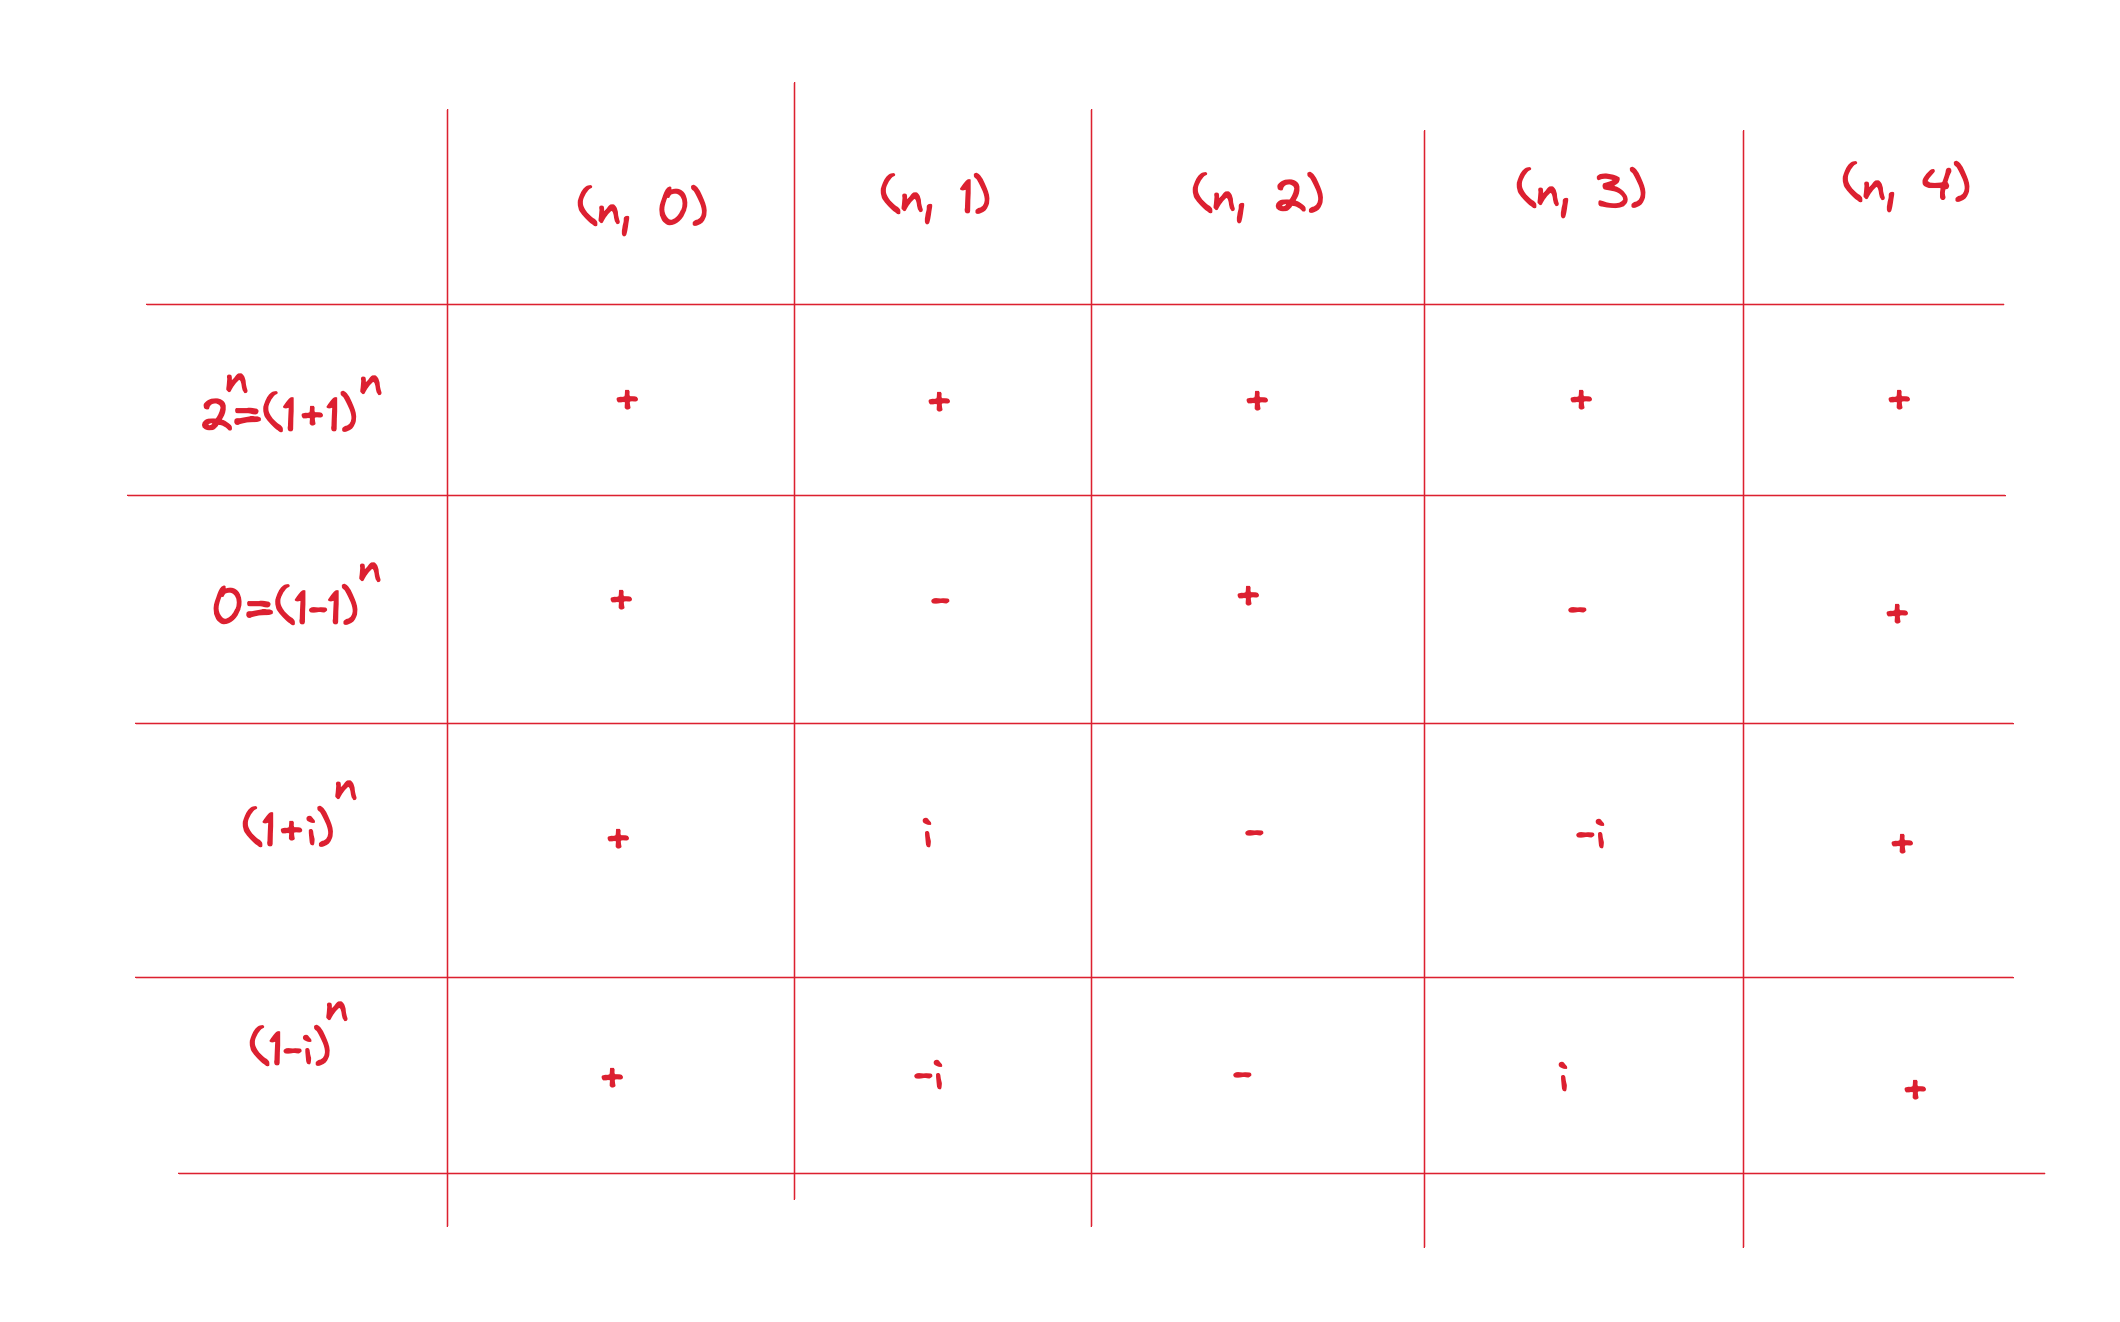
\includegraphics[width=150mm]{img}\]
	Можно представить изначальную последовательность как $\dfrac{2^n + 0 + (1 + i)^n + (1 - i)^n}{4}$ \sspace
	\textbf{8. Доказать} \sspace
	в) $\cos {\dfrac{\pi}{n}} + \cos{\dfrac{3\pi}{n}} + \cos{\dfrac{5\pi}{n}} + \cdots + \cos{\dfrac{(2n - 1)\pi}{n}}  = 0$ \sspace
	Пусть $z = |z| (\cos{\dfrac{\pi}{n}} + i\sin{\dfrac{\pi}{n}})$ \sspace
	$\cos {\dfrac{\pi}{n}} + \cos{\dfrac{3\pi}{n}} + \cos{\dfrac{5\pi}{n}} + \cdots + \cos{\dfrac{(2n - 1)\pi}{n}} = z + z^3 + z^5 + \cdots + z^{2n - 1} = z(1 + z^2 + z^4 + \cdots + z^{2n - 2}) = z\dfrac{z^{2n} - 1}{z^2 - 1} = 0$ \sspace 
	\textbf{9. Вычислить} \sspace
	з) $\sqrt[4]{-4} = \sqrt[4]{4(\cos{(\pi + 2\pi k)} + i\sin{(\pi + 2\pi k)})} = \sqrt[4]{4} (\cos{\dfrac{\pi + 2\pi k}{4}} + i \sin{\dfrac{\pi + 2\pi k}{4}}) \sspace
	$
	Корни: \sspace
	при k = 0: $\sqrt{2} (\dfrac{\sqrt{2}}{2} + i\dfrac{\sqrt{2}}{2}) = 1 + i$ \sspace
	при k = 1: $-1 + i$ \sspace
	при k = 2: $-1 - i$ \sspace
	при k = 3: $1  - i$ \sspace
	\textbf{10. Найдите все значения $z \in \mathbb{C}$ и $n \geq 2$, при которых множество $\sqrt[n]{z}$ содержит хотя бы одно действительное число.} \sspace
	$z = |z|(\cos\phi + i\sin\phi), \sqrt[n]{z} = \sqrt[n]{|z|}(\cos\dfrac{\phi}{n} + i\sin\dfrac{\phi}{n})$. Получается, что $\sin\dfrac{\phi}{n} = 0$, то есть $\dfrac{\phi}{n} = \pi k$, значит $\phi = \pi nk, k \in \mathbb{Z}$ \sspace
	Поэтому подойдут все $z: Im(z) = 0$
	 \end{document}